\documentclass{article}
\usepackage[T1]{fontenc}
\usepackage[utf8]{inputenc}
\usepackage{listings}
\usepackage{color}
\definecolor{red}{rgb}{0.6,0,0} % for strings
\definecolor{green}{rgb}{0.25,0.5,0.35} % comments
\definecolor{purple}{rgb}{0.5,0,0.35} % keywords
\definecolor{docblue}{rgb}{0.25,0.35,0.75} % javadoc
 
\lstset{
	basicstyle=\normalsize\ttfamily,
	keywordstyle=\color{purple}\bfseries,
	stringstyle=\color{red},
	commentstyle=\color{green},
	morecomment=[s][\color{docblue}]{/**}{*/},
	tabsize=4,
	showspaces=false,
	showstringspaces=false
}
	
\usepackage{graphicx}
\usepackage{fancyhdr}
\usepackage[margin=1.2in]{geometry}
\geometry{a4paper, left=20mm, right=20mm, top=20mm, bottom=20mm}
\linespread{1.5}
\begin{document}

\begin{titlepage}
	\begin{center}
		{\LARGE College of Engineering, Trivandrum}\\[3cm]
		\linespread{1.2}\huge {\bfseries Microprocessor Lab}\\[3cm]
		\linespread{1}
		
\includegraphics[width=8cm]{img/emblem.jpeg}\\[1cm]
		{\Large Gokul K\\ S5  CSE \\ Roll No: 21\\ TVE18CS021 }\\[1cm]
		\textit{ }\\[1cm]
		{\LARGE 
			Department of Computer Science\\[0.2cm]
			\today 
		}
	\end{center}
	
\end{titlepage}
\large

\newpage
\setlength{\headheight}{15.2pt}
\pagestyle{fancy}
\fancyhf{}
\fancyhead[RO]{\fontsize{12}{12}\selectfont\nouppercase\leftmark} 
\fancyhead[LO]{\fontsize{9}{12}\selectfont\nouppercase\rightmark} 

% Use the current experiment file from experiments/ folder
\section{16-bit addition using direct addressing mode}
\subsection{Aim}
To add two 16-bit numbers using direct addressing mode

\subsection{Code}
\begin{lstlisting}
DATA SEGMENT
    sum DW ?
ENDS DATA

CODE SEGMENT
ASSUME DS:DATA, CS:CODE
START:
    MOV AX, DATA
    MOV DS, AX
    MOV [1000H], 100
    MOV [1002H], 200
    MOV AX, [1000H]
    MOV BX, [1002H]
    ADD AX, BX
    MOV [sum], AX
    MOV AH, 04CH
    INT 21H
CODE ENDS
END START
\end{lstlisting}

\subsection{Output}
\begin{center}
	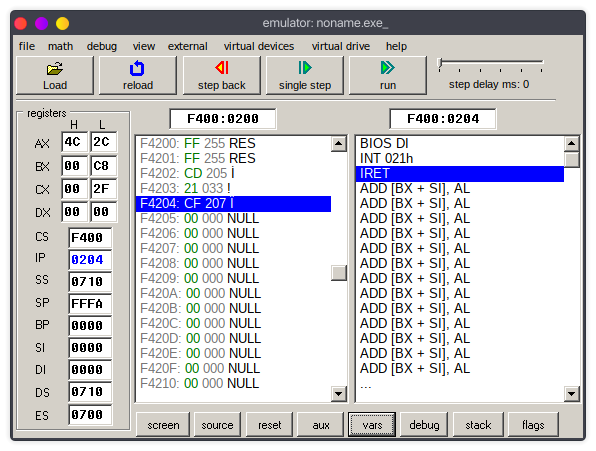
\includegraphics[width=0.90\textwidth]{img/p1/ss1.png}
	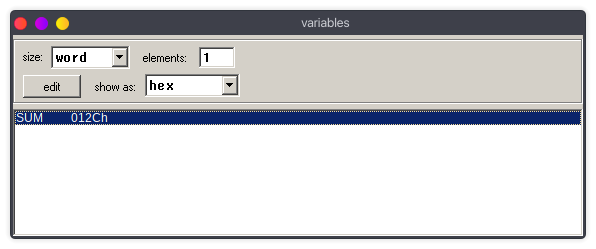
\includegraphics[width=0.90\textwidth]{img/p1/ss2.png}
\end{center}

\subsection{Result}
Two 16 bit numbers were added using direct addressing mode in emu8086 and output was verified
\newpage

\section{16-bit substraction using immediate addressing mode}
\subsection{Aim}
To substract two 16-bit numbers using immediate addressing mode

\subsection{Code}
\begin{lstlisting}
DATA SEGMENT
	difference DW ?
ENDS DATA

CODE SEGMENT
ASSUME CS:CODE, DS:DATA
START:
    MOV AX, DATA
    MOV DS, AX
    MOV AX, 200
    MOV BX, 100
    SUB AX, BX
	MOV [difference], AX
    MOV AH, 04CH
    INT 21H
CODE ENDS
END START
\end{lstlisting}

\subsection{Output}
\begin{center}
	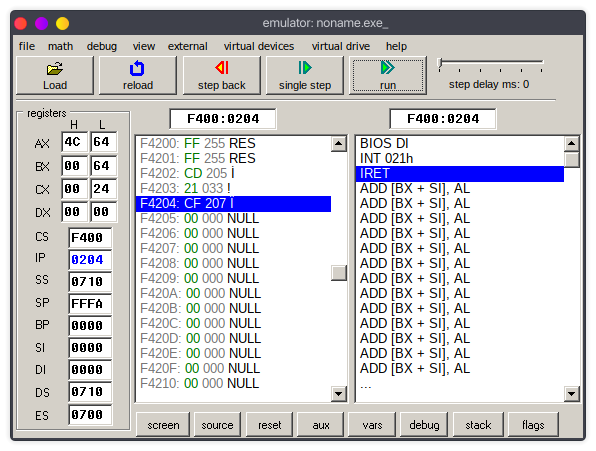
\includegraphics[width=0.90\textwidth]{img/p2/ss1.png}
	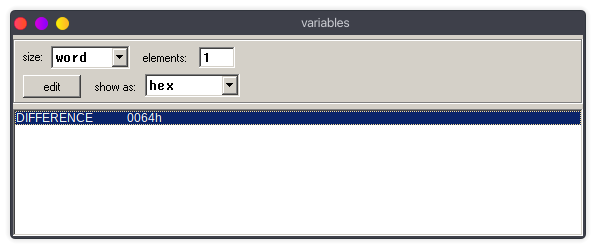
\includegraphics[width=0.90\textwidth]{img/p2/ss2.png}
\end{center}

\subsection{Result}
Two 16 bit numbers were substracted using immediate addressing mode in emu8086 and output was verified
\newpage

\section{32-bit addition}
\subsection{Aim}
To add two 32-bit numbers

\subsection{Code}
\begin{lstlisting}
DATA SEGMENT
	num1 DD 10000000H
	num2 DD 20000000H
	sum DD ?
DATA ENDS

CODE SEGMENT
ASSUME CS:CODE, DS:DATA
START:
	MOV AX, DATA
	MOV DS, AX
	MOV AX, [num1]
	MOV BX, [num2]
	ADD AX, BX
	MOV [sum], AX
	MOV AX, [num1+2]
	MOV BX, [num2+2]
	ADC AX, BX
	MOV [sum+2], AX
    MOV AH, 04CH
    INT 21H
CODE ENDS
END START
\end{lstlisting}

\subsection{Output}
\begin{center}
	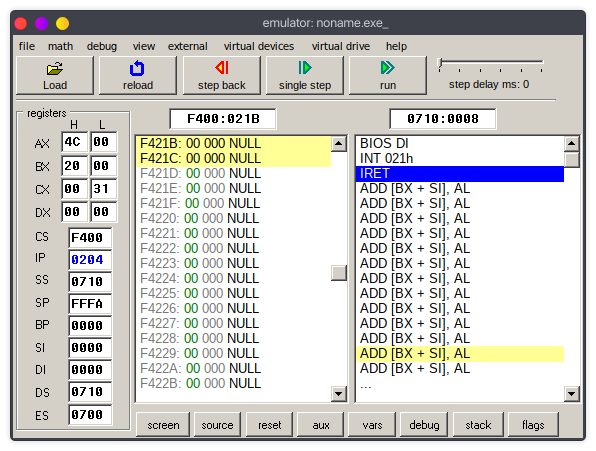
\includegraphics[width=0.90\textwidth]{img/p3/ss1.png}
	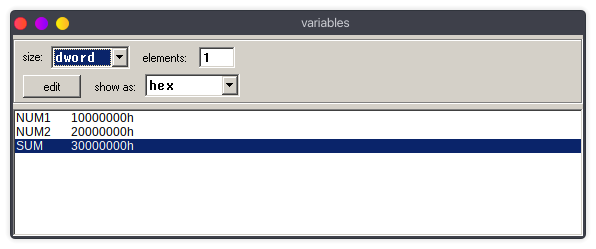
\includegraphics[width=0.90\textwidth]{img/p3/ss2.png}
\end{center}

\subsection{Result}
Two 32 bit numbers were added in emu8086 and output was verified
\newpage

\section{32-bit substraction}
\subsection{Aim}
To substract two 32-bit numbers

\subsection{Code}
\begin{lstlisting}
DATA SEGMENT
	subtrahend DD 1000H
	minuend DD 500H
	difference DD ?
ENDS DATA

CODE SEGMENT
ASSUME CS:CODE, DS:DATA
START:
	MOV AX, DATA
	MOV DS, AX
	MOV AX, [subtrahend]
	MOV BX, [minuend]
	SUB AX, BX
	MOV [difference], AX
	MOV AX, [subtrahend+2]
	MOV BX, [minuend+2]
	SUB AX, BX
	MOV [difference+2], AX
	MOV AH, 04CH
    INT 21H
ENDS CODE
END START
\end{lstlisting}

\subsection{Output}
\begin{center}
	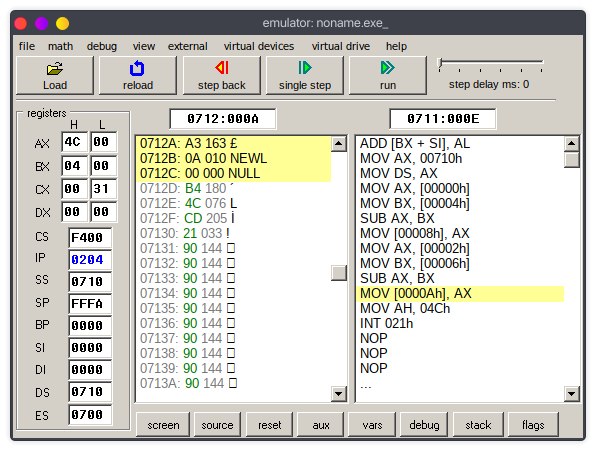
\includegraphics[width=0.90\textwidth]{img/p4/ss1.png}
	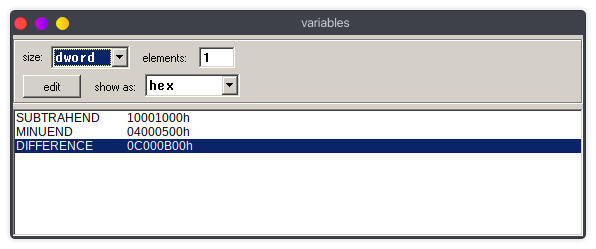
\includegraphics[width=0.90\textwidth]{img/p4/ss2.png}
\end{center}

\subsection{Result}
Two 32 bit numbers were substracted in emu8086 and output was verified
\newpage

\section{32-bit multiplication}
\subsection{Aim}
To multiply two 32-bit numbers

\subsection{Code}
\begin{lstlisting}
DATA SEGMENT
	multiplicand DW 1000H
	multiplicator DW 200H
	product DD ?
ENDS DATA 

CODE SEGMENT
ASSUME CS:CODE, DS:DATA
START:
	MOV AX, DATA
	MOV DS, AX
	MOV AX, [multiplicand]
	MUL [multiplicator]
	MOV [product], AX
	MOV [product+2], DX
    MOV AH, 04CH
    INT 21H
ENDS CODE
END START
\end{lstlisting}

\subsection{Output}
\begin{center}
	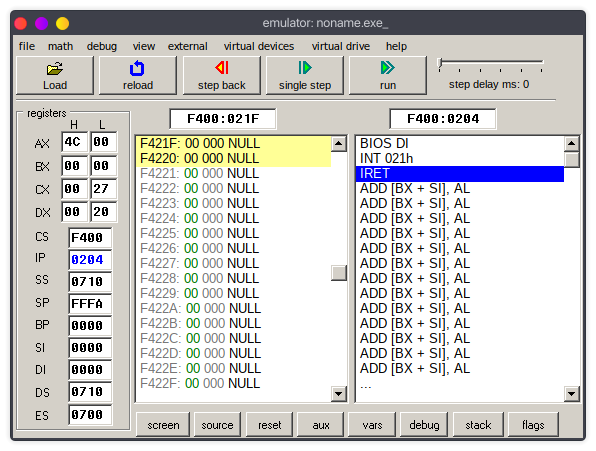
\includegraphics[width=0.90\textwidth]{img/p5/ss1.png}
	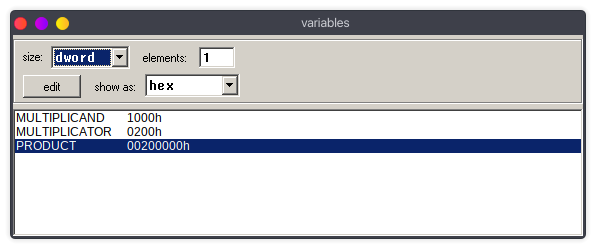
\includegraphics[width=0.90\textwidth]{img/p5/ss2.png}
\end{center}

\subsection{Result}
Two 32 bit numbers were multiplied in emu8086 and output was verified
\newpage

\section{Multiword division}
\subsection{Aim}
To divide a 32 bit number with a 16 bit number

\subsection{Code}
\begin{lstlisting}
DATA SEGMENT
	dividend DD 1000000H
	divisor DW 1000H
	quotient DD ?
	remainder DD ?
ENDS DATA

CODE SEGMENT
ASSUME CS:CODE, DS:DATA 
START:
	MOV AX, DATA
	MOV DS, AX
	MOV AX, WORD PTR [dividend+2]
	MOV BX, WORD PTR [divisor]
	DIV BX
	MOV WORD PTR [quotient+2], AX
	MOV AX, WORD PTR [dividend]
	DIV BX
	MOV WORD PTR [quotient], AX
	MOV WORD PTR [remainder], DX
	MOV AH, 04CH
    INT 21H
ENDS CODE
END START
\end{lstlisting}

\subsection{Output}
\begin{center}
	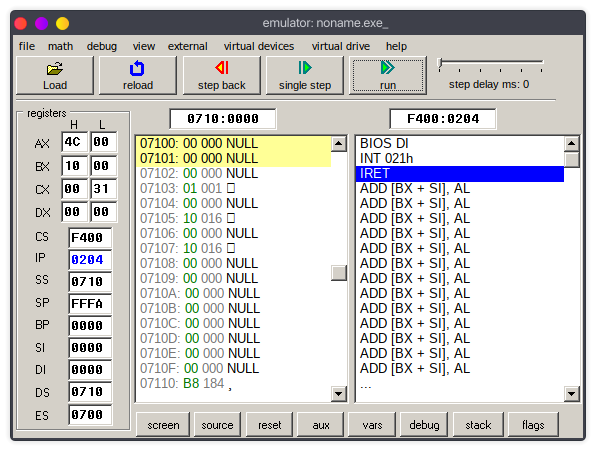
\includegraphics[width=0.90\textwidth]{img/p6/ss1.png}
	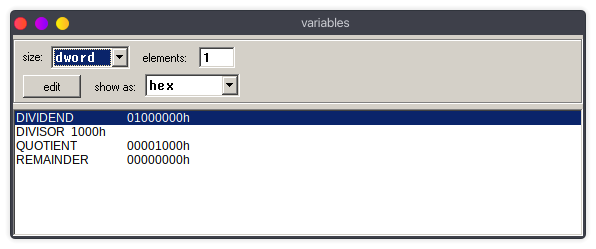
\includegraphics[width=0.90\textwidth]{img/p6/ss2.png}
\end{center}

\subsection{Result}
A 32 bit number was divided by a 16bit number in emu8086 and output was verified
\end{document}